% This is the era of digitalization and it has been observed that in past years a lot of firms ranging from small to enterprise are digitalizing their environment and processes. Here we are using the term digitalization in terms of technology and for the sake of simplicity, we can interpret the term digitalization as transforming the manual processes, information, and assets into a digital/computer-readable platform. It has started many years ago when firms have understood the significance of their data and embraced the fact that how, being stick to the non-digital environment, can lead to some serious consequences.
% \newline
% \par
% In the last decades, the technology has evolved exponentially and so is digitalization. By each passing day, we are witnessing how digitalization has revolutionized and reshape the business organizations. Every day, we are trying to discover the possible ways to digitalize our processes. Even if we look around ourselves, we can find such things in our daily work routine as well. For example, banking transactions, now we don't have to go to banks for money transfer or to inquire about the balance. Thanks to internet banking, now everything is available on the web/mobile application. This is just a simple example of digitalization in the field of banking, there are lots of other domains which have been digitalized and now serving us in the best possible way.
% \newline
% \par
% Now the question arises that does the digitalization leave the positive impact in commercial organizations as well as in our daily work routines. Organizations are investing a fortune to digitalize their processes but is it worth it? Nonetheless, we can see the advantages in almost every other sector. The communication platform has increased exponentially and is much faster and quicker. Furthermore, the transportation system like airplane and railway reservations has also drastically changed and becomes much more convenient. In other words, organizations are analyzing the regular work processes and digitalize them so that we can make the most of it.
% \newline
% \par
% So, why do we think that a digitalized environment is a core necessity for any firm? Almost in every other organization, the number of files, invoices, tax documents, etc. are increasing rapidly which they need to use very frequently in different processes. To ensure the quick and smooth run of these processes, it is very important to have faster retrieval and access to the data in such an environment. If we will leave these things to process manually, it will not only be time-consuming but also very vulnerable to human error. For example, if a person has to label any document manually, although it is very easy for them to identify the document, but if the documents are in bulk then there are fair chances of errors in some document labeling. So, to ensure an error-free environment, we need to have such a system that can handle such tasks efficiently and in less time.
% \newline
% \par
% There are many automation processes that come under the umbrella of digitalization like asset storing management, digital banking, online reservation systems, online tax return systems. One process that can be common in any system is the classification of data. Here, data can be in the form of images or documents. So, what is meant by the automatic document classification? In any system, most of the time we need to classify our data into different categories for various purposes like searching, showing relevant data according to the user's interest or any other purpose. So even in a digitalized environment, this task can be done either manually or one can think of a system where we can pass our data and it will classify and tag our documents automatically and we can clearly see which process will be more favorable for us.
% \newline
% \par
% Furthermore, we should understand that by not adapting such an environment, an organization will not only stagnate to evolve but also it will slowly affect the business as well. In previous times, companies had a dedicated team for performing these tasks manually which was not only an inefficient approach but also time-consuming. If our processes will be time-consuming and prone to errors, then how can we think of surviving in such a competitive market where every other day there is a new company come with new sets of services. This is the era of technology and each sector is leveraging the latest technologies to grow their business in the best possible way. So, if we will stick to manual processes, we will not only behind in the race but also be no more.
% \newline
% \par
% So far, we have discussed the digitalized environment, what was happening previously, how it is revolutionizing the world, why it is a must-have thing nowadays and also how can be the systems involved in the digital world. As I said, it is a very broad area and there can be different domains that we can automate. Automatic document classification is one of the end-result of a digitalized or automated process. It helps to label and identify the documents independently. Now, let's see how it can help in different ways:
% \begin{itemize}
%   \item \textbf{Time Efficient:} It is very obvious that it will reduce a lot of manual effort which will lead ultimately lead to faster processes and perhaps saving time
  
%   \item  \textbf{Less human involvement:} Since it is an automated process that requires some training via humans initially but after that this system will be independent and the teams which were previously dedicated to these tasks, can be used in other assignments.
  
%   \item \textbf{Less error rate:} We all know that the human brain can classify the documents better but when it comes to classifying the data in bulk then it is a tedious, exhaustive and time-consuming task which can cause human errors as well and ultimately lead to damage to the business. Here, an automated system eliminates all these factors and works efficiently.
  
%   \item \textbf{Long term solution:} Another benefit of this approach is that we can consider it as a long-term solution and do not have to do any extra effort because it will work for the future/upcoming data as well.
  
%   \item \textbf{Better user experience:} If we think about doing these classifications manually then it is certainly the desirable things to do, so by automating these processes will give users a better experience in terms of relaxation and time.
  
%   \item \textbf{Organization's growth:} Certainly there is a cost attached to automate such processes but this a one-time investment and if we look at the bigger picture, against that cost, the organization is saving a lot of time, resources and also faster processes which will save lot more money in the longer run.
% \end{itemize}
% \par
% The research work in the domain of document classification is itself very broad and to train a generic model for all types of documents involves a huge amount of effort and time. Since there is a specific time limit for this thesis, we are narrowing down the scope of types of documents to a limited set and in our case/problem we are dealing with tax documents. Tax documents can be income tax statement, salary slip, general receipts, invoices, disability certificates, etc. Moreover, all these documents are somewhat confidential and are not publicly available so for now due to limited time and lack of data we are just focusing on only three types which are income tax statement, salary slip, and general receipts. The thesis aims to predict the type of tax-related documents. 
% \newline
% \par
% This problem can be solved in many ways like patterns recognition, text/content analysis or image recognition but if we look closely all these methods are somehow related to the machine learning domain. So, to develop an intelligent system for this problem, we leverage the power of machine learning as it is widely used by different communities for text analysis or image recognition. Machine learning was first introduced many years ago in the 1950s but unfortunately didn't get its due popularity until 2012 when its evolution has actually started and nowadays it is being used by worldwide to solve complex problems. A lot of research has been made for training machines to learn the content from the image and have proposed many solutions but according to the results and statistics Convolutional Neural Networks which is a class of Deep Neural Networks are best suited for the problem of text analysis or image recognition and we have used the same for our problem.
% \newline
% \par
% In this paragraph, we will briefly explain the solution that we prepared for automatic document classification:
% \begin{itemize}
%   \item \textbf{Word count frequency (Non-machine learning):} This solution is based on the textual data. From the textual content, we look for meaningful keywords and categorize it according to the document types with weights. Then during the prediction, we extract the content from the document and check the keywords category and return the class which has the highest score.
  
%   \item  \textbf{Bag of Words Model with CNN:} This solution is also based on textual data. First, we extract meaningful content from the documents by filtering out stop-words and other irrelevant values. After that, we use the Keras tokenize API \cite{keras_tokenizer} to convert text data into vectors by using Bag of Word model approach \cite{bow} \cite{bow_example} as our training data for our machine learning model. For our model, we are using the Convolutional Neural Network as our machine learning model. So, for the prediction, we take the document as an input, extract the data from it then tokenize it and pass it to the predict function of the model.
  
%   \item \textbf{CNN - Transfer Learning (VGG19):} This solution is based on visual/image base data. For this, we are training Keras transfer learning model VGG19 model for three different classes. So, for the prediction, this solution takes the document as input and passes it to the predict function of the model.
% \end{itemize}
\section{Motivation}
% This thesis aims to take another step towards digitalization and to touch another domain which is being done manually and automate it. We are witnessing every day how the organizations are getting rid of their manual processes to make their services quicker and reliable to their customers. This is the need of the hour and a must-have thing for survival in the industry. In this thesis, we are choosing the manual process for the document classification which is being done by the editors and trying to automate it by leveraging state of the art machine learning techniques.
% \newline
% \par
% So, what is happening right now and what are the things that motivated us to take a step to automate this process? If we talk about the current situation, organizations have several resources as a team who are dedicatedly assigned to perform such manual tasks like labeling the organization's assets, documents, images, etc. This is not a one-time task but they have to keep performing these tasks for the upcoming documents as well. So, what are the side effects? Since the nature of this task is not interesting therefore it becomes exhausted and tiring for the editors if they have to classify or label the documents in bulk amount. Here, we can foresee the chances of human error which can be dangerous. As a technical person, we interpret this scenario as unoptimized and can be automated. Also, by this automation, we will not only optimize the current process but will save a lot of time because it will be a much faster and independent process that requires very little human interaction, which also results in less resource allocation in this domain. In short, we can make our processes quicker, cost-efficient and resource efficient.
% \newline
% \par
% So far, we have discussed how this automation is benefitting on the organization level. Let's see how it can help in the domain level and which can areas can be targeted which can leverage from this automation. Here, I would like to give a few domain examples where we can use this automated document classification solution.
% \newline
% \par
% Firstly, let's take the scenario of tax claiming process. This scenario is something where we are working and is the target of the thesis. If we see the history of this process, there were no online services or applications for the end-users to claim their tax by just sitting at home. People used to gather all their documents both the ones which are required like tax forms, attachments and also the ones which they can use for claiming tax. After the document gathering, they have to visit the tax offices and have to stand in the long queue to wait for their turn. Here, there were also the chances for the users to miss any mandatory document to submit which will result in the waste of the day sometimes. Furthermore, since there are some tax-related technicalities involved in this process, so sometimes, people who have a lack of knowledge in this domain, have to hire a lawyer or take the assistance of private firm services who can process their tax claim on their behalf. Later on, by understanding this tedious process and how much it is in demand, many tax-related consultancies firms launched online applications to claim their taxes. That was a sigh of relief to the users as they do not have to visit the tax offices anymore and can submit their tax online just by sitting at home. They just need to fill the online form and upload all the documents which are required and also the ones which can be used for tax claiming to that application and then submit it. That was an advancement in the tax consultancy domain, but the story doesn't end here. Nowadays, people are striving to more and more to make things as easier as possible. Although, the online tax return application was ease for the users but, if you take a look at the tax forms and the amount of information that users need to enter is enormous. There are several sections in tax claiming and in each section they need to enter different information like there are some sections where we have to enter the information related to the income tax statement, there is a section where we need to enter our additional expenses in the form of receipts which can be reimbursed while claiming tax etc. So, that was a long process which, sometimes later went to become a hectic thing for a user. We have realized that by only providing an online platform to the users is not enough, we also have to make it easy for them. So, to enhance the user experience further, now we thought of a system where the user just needs to upload their document and then the system will do the rest of the hectic job for the user. So what will this system exactly do? After uploading the documents to the system, it will first classify the tax-related documents automatically, extract the relevant information from the documents and then auto-fill the different sections of tax form. Now, this is something which is of great help and importance because where the users have to spend 1-2 hours to fill all the sections with the correct information, now it will just take few seconds to do the job. Here, we can see it's all about saving time and enhance the user experience more and more to make their life easier and we are hitting the right chords by using the automatic document classification solution in this domain.
% \newline
% \par
% Furthermore, another domain that I can think of is online job portals for employers. We all know that this process is a part of every type of firm. And as a job person, I have experienced difficulties several times while applying for the jobs. For example, there are some jobs where to apply there are several stages involved like first, we have to create a user account then there are some lengthy sections for personal information, information about prior work experience and companies, user's skill, etc. To be honest, if we think of it normally, a user never applies for one job at a time, instead they will take some time and apply for multiple jobs together and if for each application they have to keep filling this much information then it will not only be time-consuming but also frustrating for them and it might happen that user will end up skip that job post and moved to another which requires less time and effort. I, also personally reluctant to those applications which involve filling lengthy pieces of information because who likes it? Although there are a lot of companies that are giving a better user experience to the candidates who are applying for the jobs but, we also can't deny that there are also some companies whose job application process is very long and hectic for users. Also, I believe that by automating this process, we will not only give a favor to the job applicants but also the employer. Now the question arises how an employer can also take advantage of this solution? So, each company can have a different job application process, some companies directly ask the applicants to send their documents to their email, some companies have a full-fledged system to receive the applications but in this case, even if they have a comprehensive system, they can't really restrict the user to fill all the details as it can lead to a bad user experience, so they only mark limited information as mandatory and then upload the required documents of users. Here, we can see one common problem for the employer that after receiving the applications, they have to filter out and choose the most relevant and best candidates for their job. To do that job, they need to go through all the applications and their CVs to pick the best one. Again, this is not the optimal way to do that task and involves a lot of time, effort and resources. The user needs to upload several documents while applying for a job like CV, motivation letter, work experience letters, skilled certifications, reference letter, academic degrees, etc. What we can do here is that we can take the advantage of automated document classification to classify the user documents automatically, extract the relevant information according to their needs and show them in the most precise and presentable way in the order. It will not only make the job easy for the HR persons of the company to pick the most suitable candidates for them but also much more time efficient. 
% \newline
% \par
% Here, I would like to mention that, in previous two examples we discussed that what can be the targeted areas where we can apply the automated document classification technique to make the process faster and reliable but as you can see in the above examples, it consists of two parts, first is the document labeling/classification and the second part is text extraction. Since it is a very big problem to handle and requires a lot of time, so by understanding the limited time constraint of this thesis, we will only work on the document classification (only tax-related documents) part of the problem and the text extraction part is something which are on cards and will work on it in future. We will discuss that part in detail in Chapter \ref{chap:6}.
% \newline
% \par
% As I mentioned in the Introduction section, I have worked on three different solutions for document classification. This problem can be solved in many ways like patterns recognition, text/content analysis or image recognition but if we look closely all these methods are somehow related to the machine learning domain. So, to develop an intelligent system for this problem, we leverage the power of machine learning as it is widely used by different communities for text analysis or image recognition. Although, our main focus is to work on the machine learning-based solution but, one of my solution is not based on ML and is using simple word frequency scoring methods. Machine learning was first introduced many years ago in the 1950s but unfortunately didn't get it’s due popularity until 2012 when it’s evolution has actually started and nowadays it is being used by worldwide to solve complex problems. It has a proven track record of achieving great results in text analysis and image recognition. A lot of research has been made for training machines to learn the content from the image and have proposed many solutions but according to the results and statistics Convolutional Neural Networks \cite{url1} \cite{1708.03273}  which is a class of Deep Neural Networks \cite{Krizhevsky} are best suited for the problem of text analysis or image recognition and we have used the same for our problem.
% \newline
% \par
% If we talk about the leaning mechanism in machine learning, it works the same way as the human brain does in learning something. For example, if someone will show you an image of an object or document which you have never seen or heard about, you will definitely not be able to recognize that unless that person will tell you what it is and then you will remember that thing. But even in that case, it will be a weak memory and it's not enough information to remember that thing for a longer time. Obviously, it is because you have seen only one image of that object and it might be possible that this object can exist in different colors, positions or formats. Same can happen with a document, let's say you have never heard of a salary slip and if someone will show you a salary slip and told you what it is then maybe you somehow will be able to remember that but if next time you have to see and detect which one is a salary slip, you will look for the same pattern or format or keywords and in case of salary slips, it is fairly possible that it can exist in different formats or keywords as every company has their own format for salary slips. So, the point to understand over here is that to make our brain learn about a certain thing, we need to give or show him enough data so it can learn all the possible variations and develop a deep memory about that. The same happens in the learning process of machine learning as well, the amount and quality of data have a huge significance. To develop a well-trained model, we need to train our model with enough data with as many variations or formats as possible and in this kind of scenario, Convolutional Neural Network (CNN) is the best choice \cite{1708.03273} \cite{Krizhevsky}.
% \newline
% \par
% Since we are using Convolutional Neural Network model for this problem, let's discuss why we chose CNN and how it is feasible for that purpose. Convolutional Neural Network (ConvNet/ CNN) is a Deep Learning algorithm that mimics the human brain by accepting the image as input, learn something from that input and will be able to differentiate that image in the future. CNN is fairly popular in the domain of computer vision. It has an architecture that consists of many layers interconnected with each other and each layer stores some features from the image. Due to its very powerful architecture and huge learning capacity, it has proven to be the suitable choice for classification and that's also the reason why we chose CNN as our model.
\section{Thesis Goal}
% In this thesis, we are aiming to develop a system that can classify the document type/class of tax-related documents. We would like to break down the goals into the following:
% \newline
% \par
% \subsection{Classify Tax-related documents}
% The goal of this thesis is at the end to develop an intelligent system that can classify tax-related documents. Documents can be in the form of images or pdfs. The system will take the document as input and predict the document type. There are several classes for tax-related documents like income tax statements, salary slips, general receipts, additional expenses invoices, disability certificate, etc. Since these types of document falls in the category of personal documents and are quite confidential so there is a very limited amount of data available on the internet. Also, the open-source dataset portals don't have tax-related datasets. So, considering these things in mind, we generated the data by ourselves for limited types of documents for now which are income tax statements, salary slips, and general receipts. So, our system will only be able to predict the document of the above types.
% \newline
% \par
% \subsection{Use Machine learning and train the model}
% As I mentioned earlier, I have developed three solutions to this problem. Our main solution is based on machine learning techniques. In machine learning, there are different algorithms used based on the nature of the problem. Two major categories of machine learning algorithms are Classification and Regression. We will discuss both these types in detail in the Chapter \ref{chap:2}. For now, we can see that our problem is related to the classification category. In this solution, we have trained two different Convolution Neural Network models for multi-level classification. Although the dataset used for both models are the same but, the nature of input is different. In the first solution, we are using simple ConvNet model and we are training that model with textual data and for this, we are tokenizing the text into vector arrays and passed it to our ConvNet model. In the second solution, we are using the Keras Transfer Learning model (VGG19) which is already trained with the ImageNet dataset \cite{ILSVRC15} \cite{transfer_learning_1}. This solution is based on visual/image data. The third solution, which is not based on machine learning techniques, is using an algorithm which analyses the content of the document and based on that score the weights of the frequency of words relevant to these document types and at the end which one has the highest score, it will be the predicted document type. In the end, we will analyze the potential of each solution and based on the performance and accuracy, we would like to go with any one of them.
% \par
% \subsection{Generate Dataset}
% We all know the significance of dataset in the domain of machine learning. To develop a well-trained model, we need to have a huge amount of quality data. So, in this thesis, apart from training the model to predict the document type, we also have a high focus on the goal of data gathering or data generation. As, I mentioned earlier that in this problem, the kind of data that we are dealing with is rarely available, so we are developing a separate solution that is solely responsible for generating data. Since we have limited document types for the tax-related document, we will try to gather as many format/templates as we can for the document types and on the basis of these templates, we will generate further data.
% \par
% \subsection{Comprehensive architecture for continuous training}
% Apart from developing a system which should be able to classify tax-related document types, we also understood the need of having such a comprehensive architecture from which should be scalable and give the provision for continuous learning for our model. So, the question is why it is necessary in this case? There are two major reasons why we need such architecture.
% \begin{itemize}
%   \item \textbf{Supporting more document types:} As I mentioned earlier, there are several types of tax-related documents but due to the lack of availability of data and restricted time constraint of the thesis, we have just added three types of documents in our scope. But in the future, we have to expand the document types as soon we will have the data available. In this scenario, we want to avoid the manual mechanism required to add new type but instead, we would like to design the architecture in such a way that it will give the provision to add document type.
  
%   \item  \textbf{ Supporting more formats:} If we look at the nature of data involved in our problem, it is not restricted to exist in only one form but instead it can exist in different formats as well. For example, if we talk about the salary slip, even if the keywords in the documents are more or less the same but formats can be different, and each company has its own template. So it is pretty obvious that a single document type can be available in different formats. In this thesis, we have tried to gather a limited number of templates for the document types and we have an approach that in the future, we will gather more templates, generate the data with these formats and then add it to the existing dataset. Again, to do that, we need a provision that allows us to add more data to a particular type of document's dataset.
  
%   \item \textbf{Re-train the model:} In both the above provisions, which means after adding a new document type to the dataset or adding more data to the dataset, we need to re-train our model with the new data. So, in that case, we also need a mechanism by which we can train our model again.
% \end{itemize}
% \par
% To accommodate these provisions, we are exposing some APIs by which we can do these jobs conveniently. The below figure will help us to better visualize the architecture.
% \begin{figure}[H]
% \centering
% 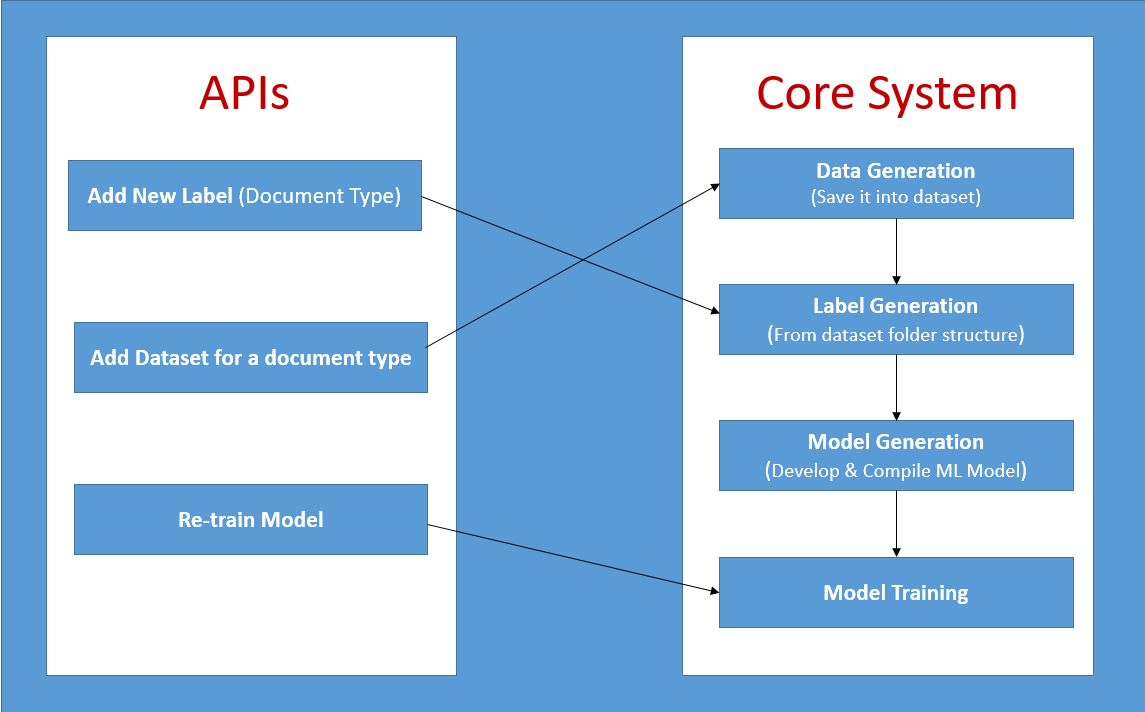
\includegraphics[scale=0.7]{images/Chapter1/API.PNG}
% \caption{API Architecture for Continuous Training}
% \label{api-arch-ct}
% \end{figure}
% \par
% \subsection{Compare solutions}
% Since we have multiple solutions for this problem which are both machine learning and non-machine learning. So, apart from the above tasks, in the end, we would like to perform some experiments by which we can analyze and compare the solutions in terms of performance, accuracy, and memory and will try to show the comparison to have a better understanding.
% \par
% Here, I would like to mention that the system will only predict based on the type of data fed to the model. Since we are focusing on only limited types of documents and also limited formats for a particular type of document so there are fair chances that our system will not be able to classify any document type and also any format for a particular document type which is not involved during the training.
\section{Related Work}
% In this section, we will discuss the research on automatic document classification being done by computer scientists. According to the research, most of the research done in this domain is mostly based on machine learning techniques. A lot of researchers and scientists have applied different machine learning algorithms or approaches for doing document classification. Some of them used textual content as a primary source of input for the classification which means they used a text classification approach to handle the problem. There are many algorithms which work very well for text classification like Support Vector Machines (SVM) \cite{svm}, Naive Bayes Classification \cite{nbc}, Neural Networks, Bag of Words (BoW) model, etc. If we talk about the algorithm used to solve this problem, then the Bag Of Words model and Convolutional Neural Network are one of the prominent techniques that were used by all. However, it is also a fact that in the domain of document classification, tax-related documents seem to be neglected by the community. Most of the researches that have been done so far is dealing with the generic documents. In further discussion, we will discuss some of the work or research done in the domain of document classification
% \par
% \subsection{Research Work I - Document Classification by Machine Learning Techniques}
% One of the research works done for the automatic document classification using Machine Learning is by Mr. Mowafy M. from Dept. of Information System Kafrelsheikh University \cite{rw1}. In this research, the approach to classifying the document is by text classification and by carried out some phases step by step. Furthermore, this research also discusses the possibility of using the Multinomial Naive Bayes with Term Frequency-Inverse document frequency (TFIDF) \cite{tfidf} method for text classification. In the end, it also compares the result of MNB TF-IDF with the KNN \cite{knn} TF-IDF method proposed by Trstenjak B, Mikac S, Donko D (2014).
% \par
% TF-IDF is a method used in text classification to calculates the weight for each term in each document. This method evaluates how important a word is to a document in a collection.
% \par
% \subsubsection{Proposed Model}
% The proposed model is developed by fusing multiple techniques like Multinomial Naive Bayes for machine learning for doing text classification, TF-IDF for text extraction and chi2 technique for feature selection. The experiment carried out for classification by breaking it into multiple tasks/phases which are Pre-processing, Training, Testing, and Usage. Below figure depicts the phases involved in the classification model:
% \begin{figure}[H]
% \centering
% 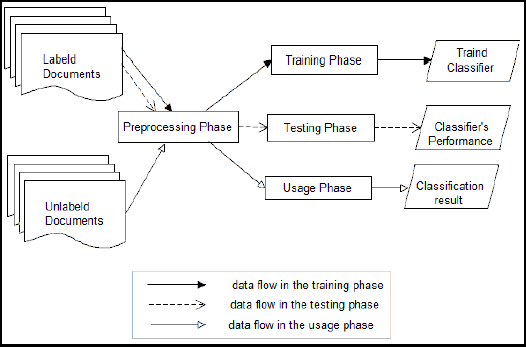
\includegraphics[scale=0.9]{images/Chapter1/RW1.PNG}
% \caption{Model Architecture \cite{rw1}}
% \label{rw1-model-arch}
% \end{figure}
% \par
% Above figure is representing the model architecture for the proposed solution. Let's deep dive into the architecture and implementation in each phase. According to the research, following are the phases:
% \begin{enumerate}
%    \item \textbf{Pre-processing:} In this phase, the input document is processed. There are two types of documents that are being used, labeled documents that are used for the training and testing phase, and unlabelled documents that are used for the usage phase. This phase is applied to both type of documents. The purpose of this phase is to make the document ready for training, testing and usage phase by removing unnecessary content from the documents. For this, they are tokenizing the documents which means converting the string into the list of tokens. After that, they are removing stop words from the tokens then applying stemming to them which converts multiple forms of words into similar canonical form.
%    \item \textbf{Training:} In this phase, they are training the classifier and in the end returning a trained classifier for classification. Following are the steps, involved in this phase:
%    \begin{itemize}
%      \item \textbf{Text Document Representation:} In this step, they are using the Bag of Word (BoW) model with the TF-IDF method for presenting the word and their number of occurrences in each document.
%      \item \textbf{Feature Selection:} This step is used to further filter out the irrelevant words from the previous input and select the most relevant feature from that. For this, they are using Chi-Square (chi2) \cite{chi2} method for feature selection.
%      \item \textbf{Training Classifier:} In this step, they are using a Multinomial Naive Bayes classifier as a model and training the model with the input from the previous step. This training classifier will be ultimately used for the testing and usage phase.
%    \end{itemize}
%    \item \textbf{Testing:} In this phase, they are testing the classifier performance by predicting unlabeled documents with the correct class and then evaluated the result.
%    \item \textbf{Usage:} By this phase, the classifier is trained and tested and now is ready to classify the documents which were not present during the training.
% \end{enumerate}
% \par
% \subsubsection{Datasets and Results}
% For this experiment, they used very famous 20-Newsgroups data by Ken Lang \cite{20_news_grp_data} which consists of 19,997 documents categorized into 20 different categories. This experiment of using the Multinomial Naive Bayes Classifier with the TF-IDF method turns out to be better than KNN with TF-IDF classification in terms of accuracy and runtime performance.
% \par
% \subsection{Research Work II - Automatic Document Classification using Machine Learning Techniques by combining textual and visual features:}
% Another piece of work/research done in the domain of automatic document classification is by Ms. Lucia Noce, a candidate for PhD. in Computer Science at the University of Insubria, Italy \cite{Noce2016DocumentIC}. Again, for this purpose, the power of machine language has been leveraged along with other tools but in this research, the approach is very sharp. As far as I have researched and seen the solution, most of the solutions for document classification are heavily relying on the textual content of the document instead of the visual information but this approach is taking the advantage of both textual and visual information and the technique is to use both information to ultimately achieve the fine-grained classification result for the documents.
% \par
% \subsubsection{Proposed Model}
% This proposed model consists of a couple of phases and uses different tools and techniques for document classification like they are using OCR for text extraction from the document and training a Convolutional Neural Network (CNN) to predict the document. The main idea of this model is to embed visually distinguishable information against the important information which may be visually indistinguishable to the documents based on the content extracted from the document to help the CNN to classify the documents easily. It is a very obvious fact that for a machine learning model, it is easier to classify visual information rather than textual information in the form of an image. According to the author, in the case of image document classification, relying just on textual or visual information can lead to intra-class similarity problem however by adding extra information we can achieve high accuracy results. The below figure represents the proposed model architecture for this research work.
% \begin{figure}[H]
% \centering
% 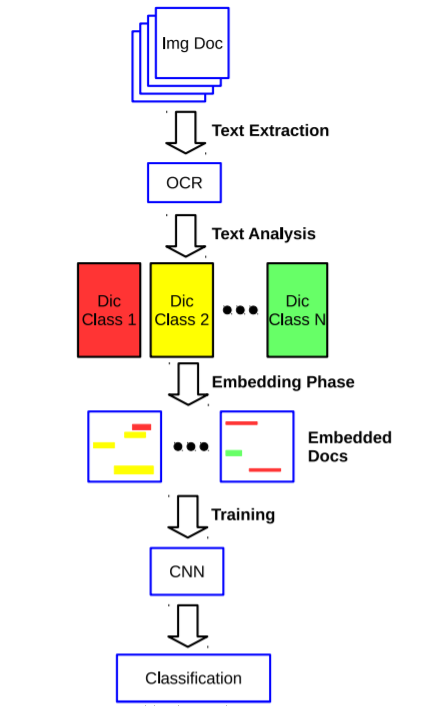
\includegraphics[scale=0.9]{images/Chapter1/RW2.PNG}
% \caption{Model Architecture \cite{Noce2016DocumentIC}}
% \label{rw2-model-arch}
% \end{figure}
% \par
% As seen in the above figure, in this model, there are three main phases involved. Let's discuss these phases in detail to know the role and contribution of each phase in the model.
% \begin{enumerate}
%    \item \textbf{Text extraction and analysis:} In this phase, documents are being processed to extract the text from the document. Optical Character Recognition (OCR) \cite{ocr} method is used for this purpose. For the sake of extracting only class relevant words or information, apart from removing stop words and stemming with the help of NLP tools, a dictionary has been built for each class which contains the representative words. To build this dictionary, all the words extracted by the OCR engine, for all the images belonging to a specific class. To build the final dictionary, they used a weighting formula. At the end of this phase, it provides a set of dictionaries for the classes which contains the relevant keyword for each class and its position coordinates that are used by the Embedding phase to underline textual information.
%     \item \textbf{Embedding:} The role of this phase to use the relevant words and position dictionaries for each class received from the previous phase and embed the textual information to the document. The purpose of doing so is to make the content information more prominent to recognize. To embed the textual information, they assigned a specific color for each class keyword and then drawn a rectangle as an information to the document using the obtained position coordinates where the rectangle is filled with the respective color against each keyword. If the keyword belongs to more than two classes, the rectangle is divided by the number of corresponding dictionaries and each part is colored by the associated class colors. These documents with marked information are used in the next phase to train the CNN model.
%      \item \textbf{Training:} In the training phase, they are training a CNN model with processed documents for the embedding phase. They implemented transfer learning using the ImageNet dataset and used the CNN model of Krizhevsky et al \cite{Krizhevsky:2017:ICD:3098997.3065386}.  During CNN training, document images are sub-sampled to fixed dimension, therefore, the text becomes unreadable; however, the marked key-word rectangles remain visible and allow the model to infer textual content.
% \end{enumerate}
% \par
% \subsubsection{Datasets and Results}
% In this experiment, they tested their model by using two different datasets "Loan Dataset" and "Tobacco Dataset". Loan Dataset consists of 14 different classes and is composed of of16250 documents in the form of document images. Out of 14 classes, they made two subsets each consists of 3 classes. The first subset (Certificate) contains the following classes: "Family Status", "Marriage Certificate" and "Residence Permit" and the second subset (Contract) contains the following classes: "Preliminary Purchase", "Loan Contract" and "Preliminary Report". The Tobacco dataset is composed of 3482 images divided into 10 classes: Advertisement, Email, Form, Letter, Memo, News, Note, Report, Resume, Scientific.
% \newline
% \par
% According to this research, it is mentioned that by using the combined approach of text and visual information, they achieved an accuracy of 79.8\% on the Tobacco dataset and 87.85\% on Loan dataset. It is also worth noting here that compared to the results of model training with the simple images with the model trained with the embedded information, the accuracy increased by 30\% for the Certificates subset and 26\% for Contracts subset which is a huge difference.
\section{Thesis Structure}
% In the subsequent chapter, the field of Machine Learning is thoroughly examined, and advanced machine learning concepts are discussed, such as Deep learning \cite{deep_learning}, precisely Artificial Neural Networks \cite{ann} and Convolution Neural Networks. Chapter 3 will comprehensively explore datasets that are being used to support this thesis. It will give insights of how images were preprocessed, what image augmentation techniques were used and which random transformations were applied on the images. Moreover, this chapter will also discuss the efficient ways that were implemented using Python Generators to read and feed small batches of data to train ConvNets instead of huge numbers, that ends up eating all the memory. In Chapter 4, all the pretrained and predefined Convolution Neural Networks models involved that eventually helped propose a custom network will be discussed. Chapter 5 will discuss the implementation of proposed ConvNets in details, how they were trained and which techniques were used. In this chapter, the experiments that were carried out and their results will be described. All those results will be further evaluated by numerous metrics and graphs. In the last section, that is Chapter 6, all the work done for this thesis will be summarized and will discuss what was learned and if this thesis helped in solving described problem or at least have given some directions. Lastly, discussion on future work will be presented followed by any tasks that were planned but didn't finish due to time constraints.